\documentclass[11pt,letterpaper]{article}
\usepackage[margin=2.5cm,top=3.5cm,bottom=3cm]{geometry}
\usepackage{booktabs}
\usepackage{graphicx}
\usepackage[hidelinks]{hyperref}
\usepackage{microtype}
\usepackage[table,dvipsnames]{xcolor}
\usepackage{longtable}
\usepackage{array}
\usepackage{caption}
\usepackage[T1]{fontenc}
\usepackage{lmodern}
\usepackage{fancyhdr}
\usepackage{amsmath}
\usepackage{titlesec}
\usepackage{enumitem}

\definecolor{wavblue}{RGB}{26,58,92}
\definecolor{wavgray}{RGB}{120,120,120}
\definecolor{wavlight}{RGB}{235,242,250}
\definecolor{wincolor}{RGB}{0,110,0}

\graphicspath{{/Users/egs/repos/waverider/benchmarks/canonical_tests/}}

\pagestyle{fancy}
\fancyhf{}
\fancyhead[L]{\small\color{wavgray}Manifold-Informed Architecture Benchmark \textemdash\ TINY\_IMAGENET}
\fancyhead[R]{\small\color{wavgray}\texttt{waverider @ 4b8002e}}
\fancyfoot[C]{\small\color{wavgray}\thepage}
\renewcommand{\headrulewidth}{0.4pt}

\titleformat{\section}{\large\bfseries\color{wavblue}}{}{0em}{}[\color{wavblue}\titlerule]
\titleformat{\subsection}{\normalsize\bfseries\color{wavblue}}{}{0em}{}
\setlength{\parindent}{0pt}
\setlength{\parskip}{4pt plus 1pt}

\begin{document}

\begin{center}
  {\LARGE\bfseries\color{wavblue} Manifold-Informed Architecture Benchmark}\\[6pt]
  {\large TINY\_IMAGENET: 200 classes, 12,288D input}\\[8pt]
  {\small Generated: 2026-04-14 20:54:37 \quad$|$\quad Apple M5 Max MacBook Pro, 64 GB RAM, 2TB SSD}\\[2pt]
  {\small\texttt{waverider @ 4b8002e} (--abbrev-re
4b8002ee9a2e3d56a219d7dab695a80b8efd1e07) \quad$|$\quad 2026-04-14 20:51:52 -0400}
\end{center}
{\color{wavblue}\noindent\rule{\linewidth}{1.5pt}}
\medskip

\noindent\colorbox{wavlight}{\parbox{\dimexpr\linewidth-2\fboxsep\relax}{
  \smallskip
  \textbf{Best:} Intrinsic Dim (PCA$\rightarrow$200D$\rightarrow$output)\quad test acc $= 0.0336 \pm 0.0012$\\[2pt]
  \textbf{vs Standard:} $+0.0070$ (0.70\,pp)\quad 164.3$\times$ fewer params\quad 207.8$\times$ acc/Kparam\\[2pt]
  \textbf{Manifold:} 12,288D $\rightarrow$ 20D (99.8\%\ noise dimensions)\\[2pt]
  \smallskip
}}
\bigskip

\section{Experimental Setup}

\begin{tabular}{@{}ll@{}}
\toprule
\textbf{Parameter} & \textbf{Value} \\
\midrule
  Dataset & TINY\_IMAGENET \\
  Input dimensionality & 12,288D \\
  Classes & 200 \\
  Intrinsic dim ($d$) & 20 \\
  Variance threshold ($\tau$) & 0.9 \\
  Epochs & 50 \\
  Trials & 3 \\
\bottomrule
\end{tabular}

\section{Manifold Discovery}

Local PCA over the training set, $k = ?$ neighbors. Intrinsic dimensionality $d$ is taken as the maximum per-class maximum at $\tau = 0.9$, clamped to $n_{\mathrm{classes}} = 200$.

\begin{tabular}{@{}rrrrrr@{}}
\toprule
$\tau$ & Mean $d$ & Std & Min & Max & Noise (\%) \\
\midrule
  0.95 & 19.6 & 0.8 & 17 & 21 & 99.8 \\
  0.90 & 16.6 & 0.9 & 14 & 18 & 99.9 \\
  0.85 & 14.2 & 1.0 & 11 & 16 & 99.9 \\
  0.80 & 12.3 & 1.0 & 9 & 14 & 99.9 \\
\bottomrule
\end{tabular}

\subsection{Per-Class Intrinsic Dimensionality}

Showing the 10 highest- and 10 lowest-dimensional classes of 200 total, sorted by mean $d$.

\begin{tabular}{@{}lrrrr@{}}
\toprule
Class & Mean $d$ & Std & Min & Max \\
\midrule
  146 & 20.0 & 0.0 & 20 & 20 \\
  55 & 19.9 & 0.3 & 19 & 20 \\
  13 & 19.5 & 0.5 & 19 & 20 \\
  99 & 19.5 & 0.5 & 19 & 20 \\
  108 & 19.5 & 0.5 & 19 & 20 \\
  173 & 19.2 & 0.4 & 19 & 20 \\
  90 & 19.1 & 0.3 & 19 & 20 \\
  147 & 19.1 & 0.7 & 18 & 20 \\
  152 & 19.1 & 0.3 & 19 & 20 \\
  16 & 19.0 & 0.4 & 18 & 20 \\
  \multicolumn{5}{c}{\ldots} \\
  20 & 15.6 & 1.2 & 14 & 17 \\
  4 & 15.5 & 0.7 & 14 & 16 \\
  179 & 15.5 & 0.8 & 14 & 17 \\
  186 & 15.5 & 0.9 & 14 & 17 \\
  48 & 15.4 & 0.7 & 14 & 16 \\
  161 & 15.2 & 0.9 & 14 & 17 \\
  94 & 15.1 & 0.5 & 14 & 16 \\
  153 & 14.9 & 0.7 & 14 & 16 \\
  116 & 14.7 & 0.5 & 14 & 15 \\
  187 & 14.6 & 1.2 & 13 & 16 \\
\bottomrule
\end{tabular}

\section{Architecture Comparison}

{\small
\begin{tabular}{@{}p{7cm}rccr@{}}
\toprule
\textbf{Architecture} & \textbf{Params} & \textbf{Test Acc ($\mu \pm \sigma$)} & \textbf{Loss} & \textbf{Acc/Kparam} \\
\midrule
  {Standard (1024$\rightarrow$512)} & 13,211,336 & $0.0266 \pm 0.0010$ & 4565.6958 & 0.0000 \\
  {Wide Manifold (d+1, d=200)} & 2,510,489 & $0.0241 \pm 0.0019$ & 64.0025 & 0.0000 \\
  {Manifold (d=200)} & 2,498,000 & $0.0260 \pm 0.0023$ & 69.4988 & 0.0000 \\
  {ManifoldAdam (1024$\rightarrow$512, proj$\rightarrow$200D)} & 13,211,336 & $0.0264 \pm 0.0008$ & 3297.0621 & 0.0000 \\
  {PCA$\rightarrow$200D + MLP (2d$\rightarrow$d)} & 200,800 & $0.0279 \pm 0.0025$ & 228.4910 & 0.0001 \\
  {\color{wincolor}Intrinsic Dim (PCA$\rightarrow$200D$\rightarrow$output)\,$\star$} & 80,400 & $0.0336 \pm 0.0012$ & 6.8843 & 0.0004 \\
\bottomrule
\end{tabular}
}

\smallskip
{\small $\star$ = best performing architecture}

\section{Key Findings}

\begin{itemize}[leftmargin=*,itemsep=3pt]
  \item \textbf{Best architecture:} Intrinsic Dim (PCA$\rightarrow$200D$\rightarrow$output) \textemdash\ test accuracy $0.0336 \pm 0.0012$
  \item \textbf{vs Standard:} $+0.0070$ (0.70\,pp) accuracy gain
  \item \textbf{Parameter reduction:} 164.3$\times$ fewer parameters (80,400 vs 13,211,336)
  \item \textbf{Parameter efficiency:} 207.8$\times$ improvement (0.0004 vs 0.0000 acc/Kparam)
  \item \textbf{Manifold compression:} 12,288D $\rightarrow$ 20D (99.8\%\ of ambient dimensions carry no structure)
\end{itemize}

\clearpage
\section{Result Figure}

\begin{figure}[htbp]
\centering
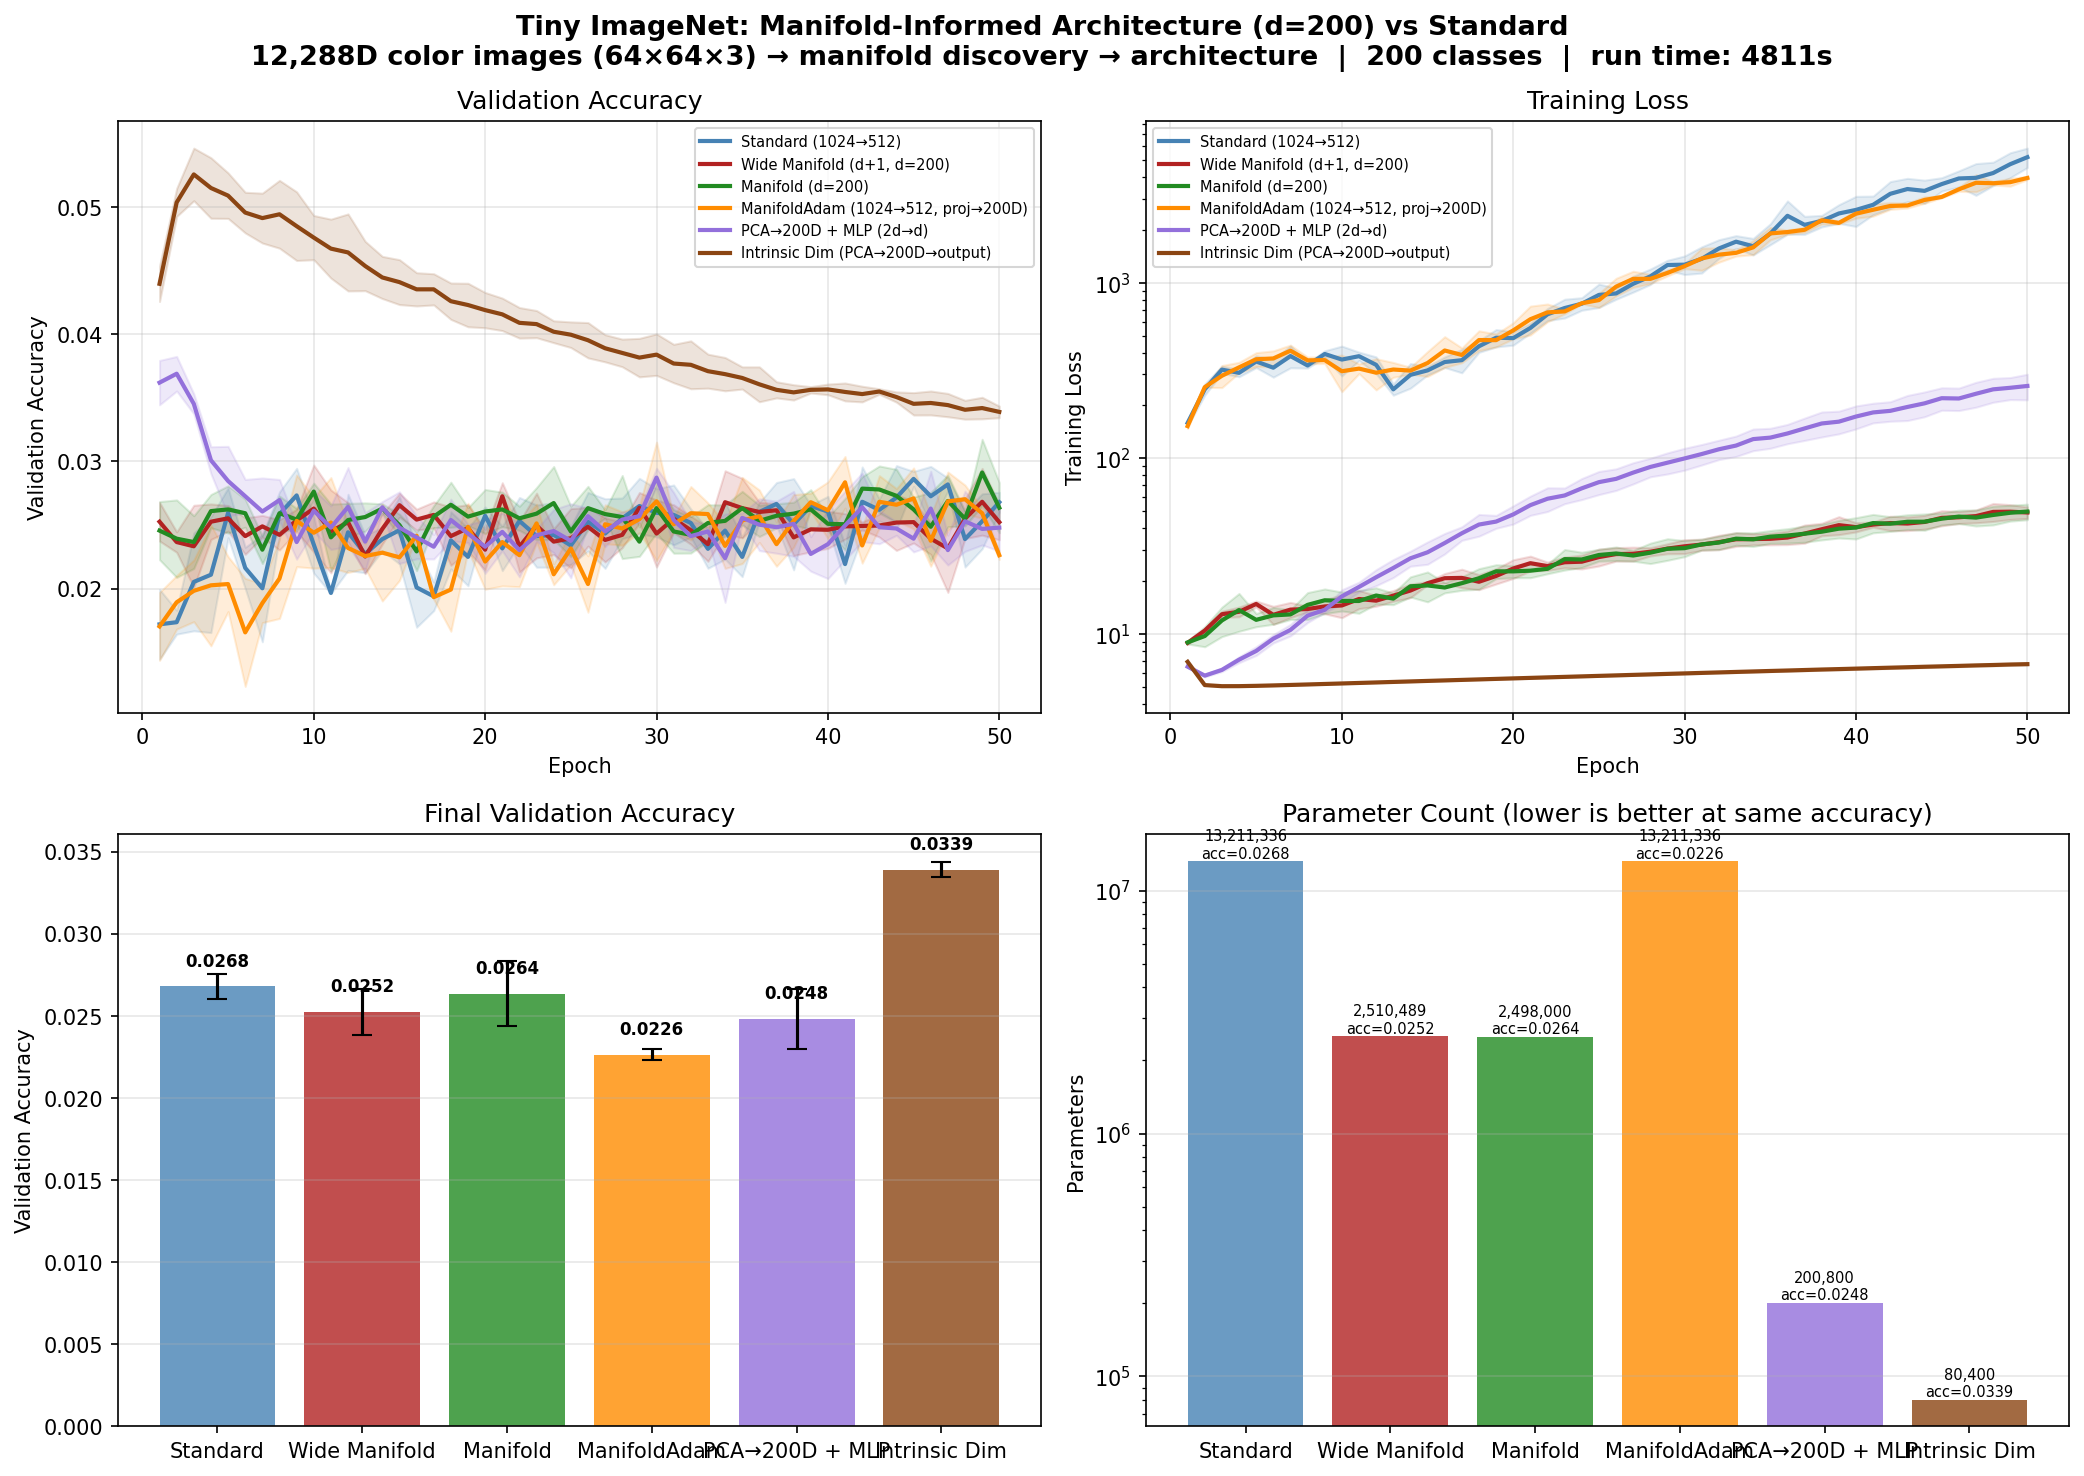
\includegraphics[width=\textwidth]{tiny_imagenet_architecture_results}
\caption{TINY\_IMAGENET manifold-informed vs.\ standard architecture comparison. $d = 20$, 50 epochs, 3 trials.}
\end{figure}

\section{Provenance}

\begin{tabular}{@{}ll@{}}
\toprule
\textbf{Item} & \textbf{Value} \\
\midrule
  Repository & \href{https://github.com/Flux-Frontiers/waverider}{Flux-Frontiers/waverider} \\
  Commit & \texttt{4b8002e} (--abbrev-re
4b8002ee9a2e3d56a219d7dab695a80b8efd1e07) \\
  Commit date & 2026-04-14 20:51:52 -0400 \\
  Commit message & add: cifar10 results \\
  Python & 3.12.13 \\
  TensorFlow & 2.16.2 \\
  Device & GPU \\
  Host & Turing \\
  OS & macOS-26.4-arm64-arm-64bit \\
  Machine & Apple M5 Max MacBook Pro, 64 GB RAM, 2TB SSD \\
  Generated & 2026-04-14 20:54:37 \\
\bottomrule
\end{tabular}

\end{document}
